\documentclass[tikz,border=5pt]{standalone}
\usepackage{tikz}
\usetikzlibrary{arrows.meta,angles,quotes}
\definecolor{nebula}{HTML}{6366F1}
\definecolor{spark}{HTML}{14B8A6}
\definecolor{ink}{HTML}{334155}
\begin{document}
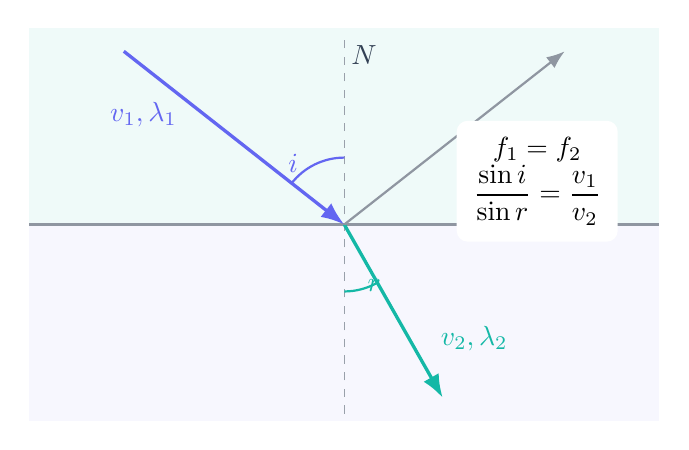
\begin{tikzpicture}[font=\sffamily,>=Latex]
  \fill[nebula!5] (-4,-2.5) rectangle (4,0);
  \fill[spark!7] (-4,0) rectangle (4,2.5);
  \draw[very thick,ink!55] (-4,0)--(4,0);
  \draw[dashed,ink!50] (0,-2.4)--(0,2.4);
  \draw[->,very thick,nebula] (-2.8,2.2)--(0,0);
  \draw[->,very thick,spark] (0,0)--(1.25,-2.2);
  \draw[->,thick,ink!55] (0,0)--(2.8,2.2);
  \draw[nebula,thick] (0,0.85) arc[start angle=90,end angle=142,radius=.85];
  \draw[spark,thick] (0,-.85) arc[start angle=-90,end angle=-60,radius=.85];
  \node[nebula] at (-.65,.78) {$i$};
  \node[spark] at (.38,-.78) {$r$};
  \node[ink] at (.25,2.15) {$N$};
  \node[nebula] at (-2.55,1.4) {$v_1,\lambda_1$};
  \node[spark] at (1.65,-1.45) {$v_2,\lambda_2$};
  \node[align=center,fill=white,rounded corners=4pt,inner sep=6pt] at (2.45,.55) {$f_1=f_2$\\$\displaystyle\frac{\sin i}{\sin r}=\frac{v_1}{v_2}$};
\end{tikzpicture}
\end{document}
